\documentclass[11pt,a4paper,english]{article} %document type and language
\usepackage[utf8]{inputenc}	% set character set to support some UTF-8
\usepackage{babel} 	% multi-language support
% \usepackage{sectsty}	% allow redefinition of section command formatting
\usepackage{tabularx}	% more table options
\usepackage{titling}	% allow redefinition of title formatting
\usepackage{imakeidx}	% create and index of words
\usepackage{xcolor}	% more color options
\usepackage{enumitem}	% more list formatting options
\usepackage{tocloft}	% redefine table of contents, new list like objects

\usepackage[centering,noheadfoot,margin=1in]{geometry}

%set TOC margins
\setlength{\cftbeforesecskip}{15pt} % skip in TOC

% remove paragraph white space and modify space between list items
\usepackage{parskip}

% Set font globally
\usepackage{lmodern}                % load Latin modern fonts
\usepackage[defaultsans]{cantarell} % cantarell fonts

% HACK: https://tex.stackexchange.com/questions/58087/how-to-remove-the-warnings-font-shape-ot1-cmss-m-n-in-size-4-not-available
\usepackage{anyfontsize}

% set LaTeX global font
\renewcommand{\familydefault}{\sfdefault}
\renewcommand{\sfdefault}{lmss}

% set styling headings
%\allsectionsfont{\usefont{OT1}{phi}{b}{n}}

\usepackage{float} 	% floats
\usepackage{graphicx}	% Graphics
\usepackage{amsmath}	% extensive math options
\usepackage{amssymb}	% special math symbols
\usepackage[Gray,squaren,thinqspace,thinspace]{SIunits} % elegant units
\usepackage{listings}                                   % source code

% Custom Operators
%% Expectation symbol
\DeclareMathOperator*{\E}{\mathbb{E}}
\DeclareMathOperator*{\Cov}{\mathrm{Cov}}
\DeclareMathOperator*{\Var}{\mathrm{Var}}

% missing math commands
\providecommand{\abs}[1]{\left\lvert#1\right\rvert}                    % |.|
\providecommand{\br}[1]{\left(#1\right)}                               % (.)
\providecommand{\sbr}[1]{\left[#1\right]}                              % [.]
\providecommand{\ddfrac}[2]{\frac{\displaystyle #1}{\displaystyle #2}}
% use \math rm{d} to include math differential

% independence symbol
% https://tex.stackexchange.com/questions/79434/double-perpendicular-symbol-for-independence
\newcommand{\indep}{\perp\!\!\!\!\perp}


% options for listings
\lstset{
  breaklines=true,
  postbreak=\raisebox{0ex}[0ex][0ex]{\ensuremath{\color{red}\hookrightarrow\space}},
  numbers=left,
  numbersep=5pt,
  numberstyle=\tiny\color{gray},
  basicstyle=\footnotesize\ttfamily
}

% NEEDS to be before hyperref, cleveref and autonum
% number figures, tables and equations within the sections
\numberwithin{equation}{section}
\numberwithin{figure}{section}
\numberwithin{table}{section}

% references and annotation, citations
\usepackage[small,bf,hang]{caption}        % captions
\usepackage{subcaption}                    % adds sub figure & sub caption
\usepackage{sidecap}                       % adds side captions
\usepackage{hyperref}                      % add hyperlinks to references
\usepackage[noabbrev,nameinlink]{cleveref} % better references than default~\ref
% Hack:https://tex.stackexchange.com/questions/285950/package-autonum-needs-the-obsolete-etex-package
\expandafter\def\csname ver@etex.sty\endcsname{3000/12/31}
\let\globcount\newcount
% \usepackage{autonum}                       % only number referenced equations
\usepackage{url}                           % URLs
\usepackage{cite}                          % well formed numeric citations

% biblatex for references
% \usepackage{biblatex}
% \addbibresource{literature.bib}
% csquotes recommended: https://tex.stackexchange.com/questions/229638/package-biblatex-warning-babel-polyglossia-detected-but-csquotes-missing
% \usepackage{csquotes}

% format hyperlinks
\colorlet{linkcolour}{black}
\colorlet{urlcolour}{blue}
\hypersetup{colorlinks=true,
            linkcolor=linkcolour,
            citecolor=linkcolour,
            urlcolor=urlcolour}

%\usepackage{todonotes} % add to do notes
\usepackage{epstopdf}  % process eps-images
\usepackage{float}     % floats
\usepackage{fancyhdr}  % header and footer
% HACK: https://tex.stackexchange.com/questions/664532/fancyhr-warning-footskip-is-too-small
\setlength{\footskip}{14pt}

% default path for figures
\graphicspath{{figures/}}

% If we have multiple directories, specify them like this: \graphicspath{{figures_ch1/}{figures_ch2/}}.

% For rendering tikz
\usepackage{pgfplots}
\pgfplotsset{compat=1.18}
\usetikzlibrary{decorations.pathreplacing} % Load the library for drawing braces


% Define some math environments
\usepackage{amsthm}

\newtheorem{theorem}{Theorem}[section]
\newtheorem{corollary}{Corollary}[theorem]
\newtheorem{lemma}[theorem]{Lemma}

\theoremstyle{definition}
\newtheorem{definition}{Definition}[section]

\theoremstyle{remark}
\newtheorem*{remark}{Remark}

% set header and footer
\pagestyle{fancy}
\fancyhf{}                           % clear all header and footer fields
\cfoot{\thepage}                     % add page number
\renewcommand{\headrulewidth}{0pt} % add horizontal line of 0.4pt thick

\title{Linear Programming Relaxation for Inference}
\author{Julian Budde}
\date{\today}
\begin{document}

\maketitle

\paragraph{Goal} Inference for the \textit{value} (or cost) of a linear program.

\paragraph{Main Idea} The value function of the linear program typically exhibits kinks (i.e.~point of non-differentiability) when viewed as a function of the underlying parameters.
This renders typical inference approaches --- like the non-parametric bootstrap --- invalid.
Instead of constructing confidence intervals based on estimators of the value function directly, we perform inference using a conservative, but smooth approximation.
For the smooth approximation we can use standard approaches.

\section{Illustration of the Idea}

We want to perform inference on the value function of a linear program.
To begin, let's consider the two-dimensional case.

\begin{equation}
	\min_{x\in [0,1]^2} c'x.
\end{equation}
Here, $x$ are the choice variables, $c$ is a coefficient vector, and the constraints are implicit in the restriction $x \in [0,1]^2$.
In standard form these are four constraints, namely $x \leq 0, -x \leq 0$, where inequalities are component-wise.

The feasible region is a unit square centered at $(0.5, 0.5)$. Solutions are unique as long as $c$ has no $0$-entry.
If $c=\mathbf{0}$, all $x\in [0,1]^2$ are optimal. If either $c_j = 0, c_i\neq0$, there are infinitely many solutions with $c_j \in [0,1]$.
Whenever $c_1\neq0, c_2\neq0$ we have a unique solution that appears at one of the corners of $[0,1]^2$ depending on the signs of $c_1, c_2$.

Assume $c_i, c_j \neq 0$ so we have a unique solution.
Figure~\ref{fig:feasible_dim_2} plots the feasible region for various constraints in $\mathbb{R}^2$ and the value functions as a function of $c_1$ with $c_2=0.5$ fixed.
The blue square is the box constraint $x\in[0,1]^2$.
The associated value function exhibits a clear kink at $c_1 = 0$.

Now the idea is, to slightly enlarge the box $[0,1]^2$ to a set $\mathcal{A}$ that is strictly convex.
A first natural idea is the circle centered at $(0.5, 0.5)$ with radius $r=0.5$.
This set is defined by $\mathcal{A} = \{x \in \mathbb{R}^2: (x_1 - 0.5)^2 + (x_2 - 0.5)^2 \leq 0.5\}$.

The resulting program is
\begin{equation}
	\min_{x\in\mathcal{A}} c'x,
\end{equation}
which is no longer a linear program, since the constraint is not linear.
However, this is a convex optimization problem for which solution methods exist in general.
\footnote{In fact, it has an easy to characterize analytical solution that can be derived using a Lagrangian.}

Since the feasible region is larger, the value function lies below the value function of the linear program.
Also, the solution no longer features a kink.
Intuitively, solutions are now at points of tangency between the level curves of the objective and and the border of the circle.
Since we smoothed out the edges, points of tangency now continuously change when $c$ changes.
So solutions are still at the extreme points but now there are infinitely many, not four of them.

However, the solutoin is visibly smaller (or in our interpretation: conservative).
So maybe $\mathcal{A}$ is too large a relaxation to be useful.

Another way to construct a tighter strictly convex set containing $[0,1]^2$ is the following.
The idea is to use a higher order polynomial that comes closer to a square with slightly rounded out corners.
We can then either use sets defined by inequalities of the following form
\begin{equation*}
	(x_1-0.5)^k + (x_2-0.5)^k \leq c
\end{equation*}
where $c\in\mathbb{R}$ is a constant given by $c = (1-0.5)^k + (1-0.5)^k$ that ensures the unit square is included.
Or, we additionally shift multiple of these sets and take their intersections, which gives a smaller final set for the same order polynomial.
Take the four sets defined by the following four inequalities. For example,
\begin{align}
	& (x_1 - c')^4 + (x_2 - 0.5) \leq 0.5, \\
	& (x_1 - (1-c'))^4 + (x_2 - 0.5) \leq 0.5, \\
	& (x_1 - 0.5)^4 + (x_2 - c') \leq 0.5, \\
	& (x_1 - 0.5)^4 + (x_2 - (1-c')) \leq 0.5,
\end{align}
where again $c'$ ensures $[0,1]^2$ is included.

Figure~\ref{fig:feasible_dim_2} plots the first option for $k\in\{2,4,6,10\}$.
The feasible region shrinks towards the unit square as $k$ increases.
Hence, the value function is also closer to the original linear program one, while still being smooth.

\begin{figure}
	\centering
	\caption{Feasible Regions and Value Functions in $\mathbb{R}^2$.}\label{fig:feasible_dim_2}

	\begin{subfigure}{0.9\textwidth}
		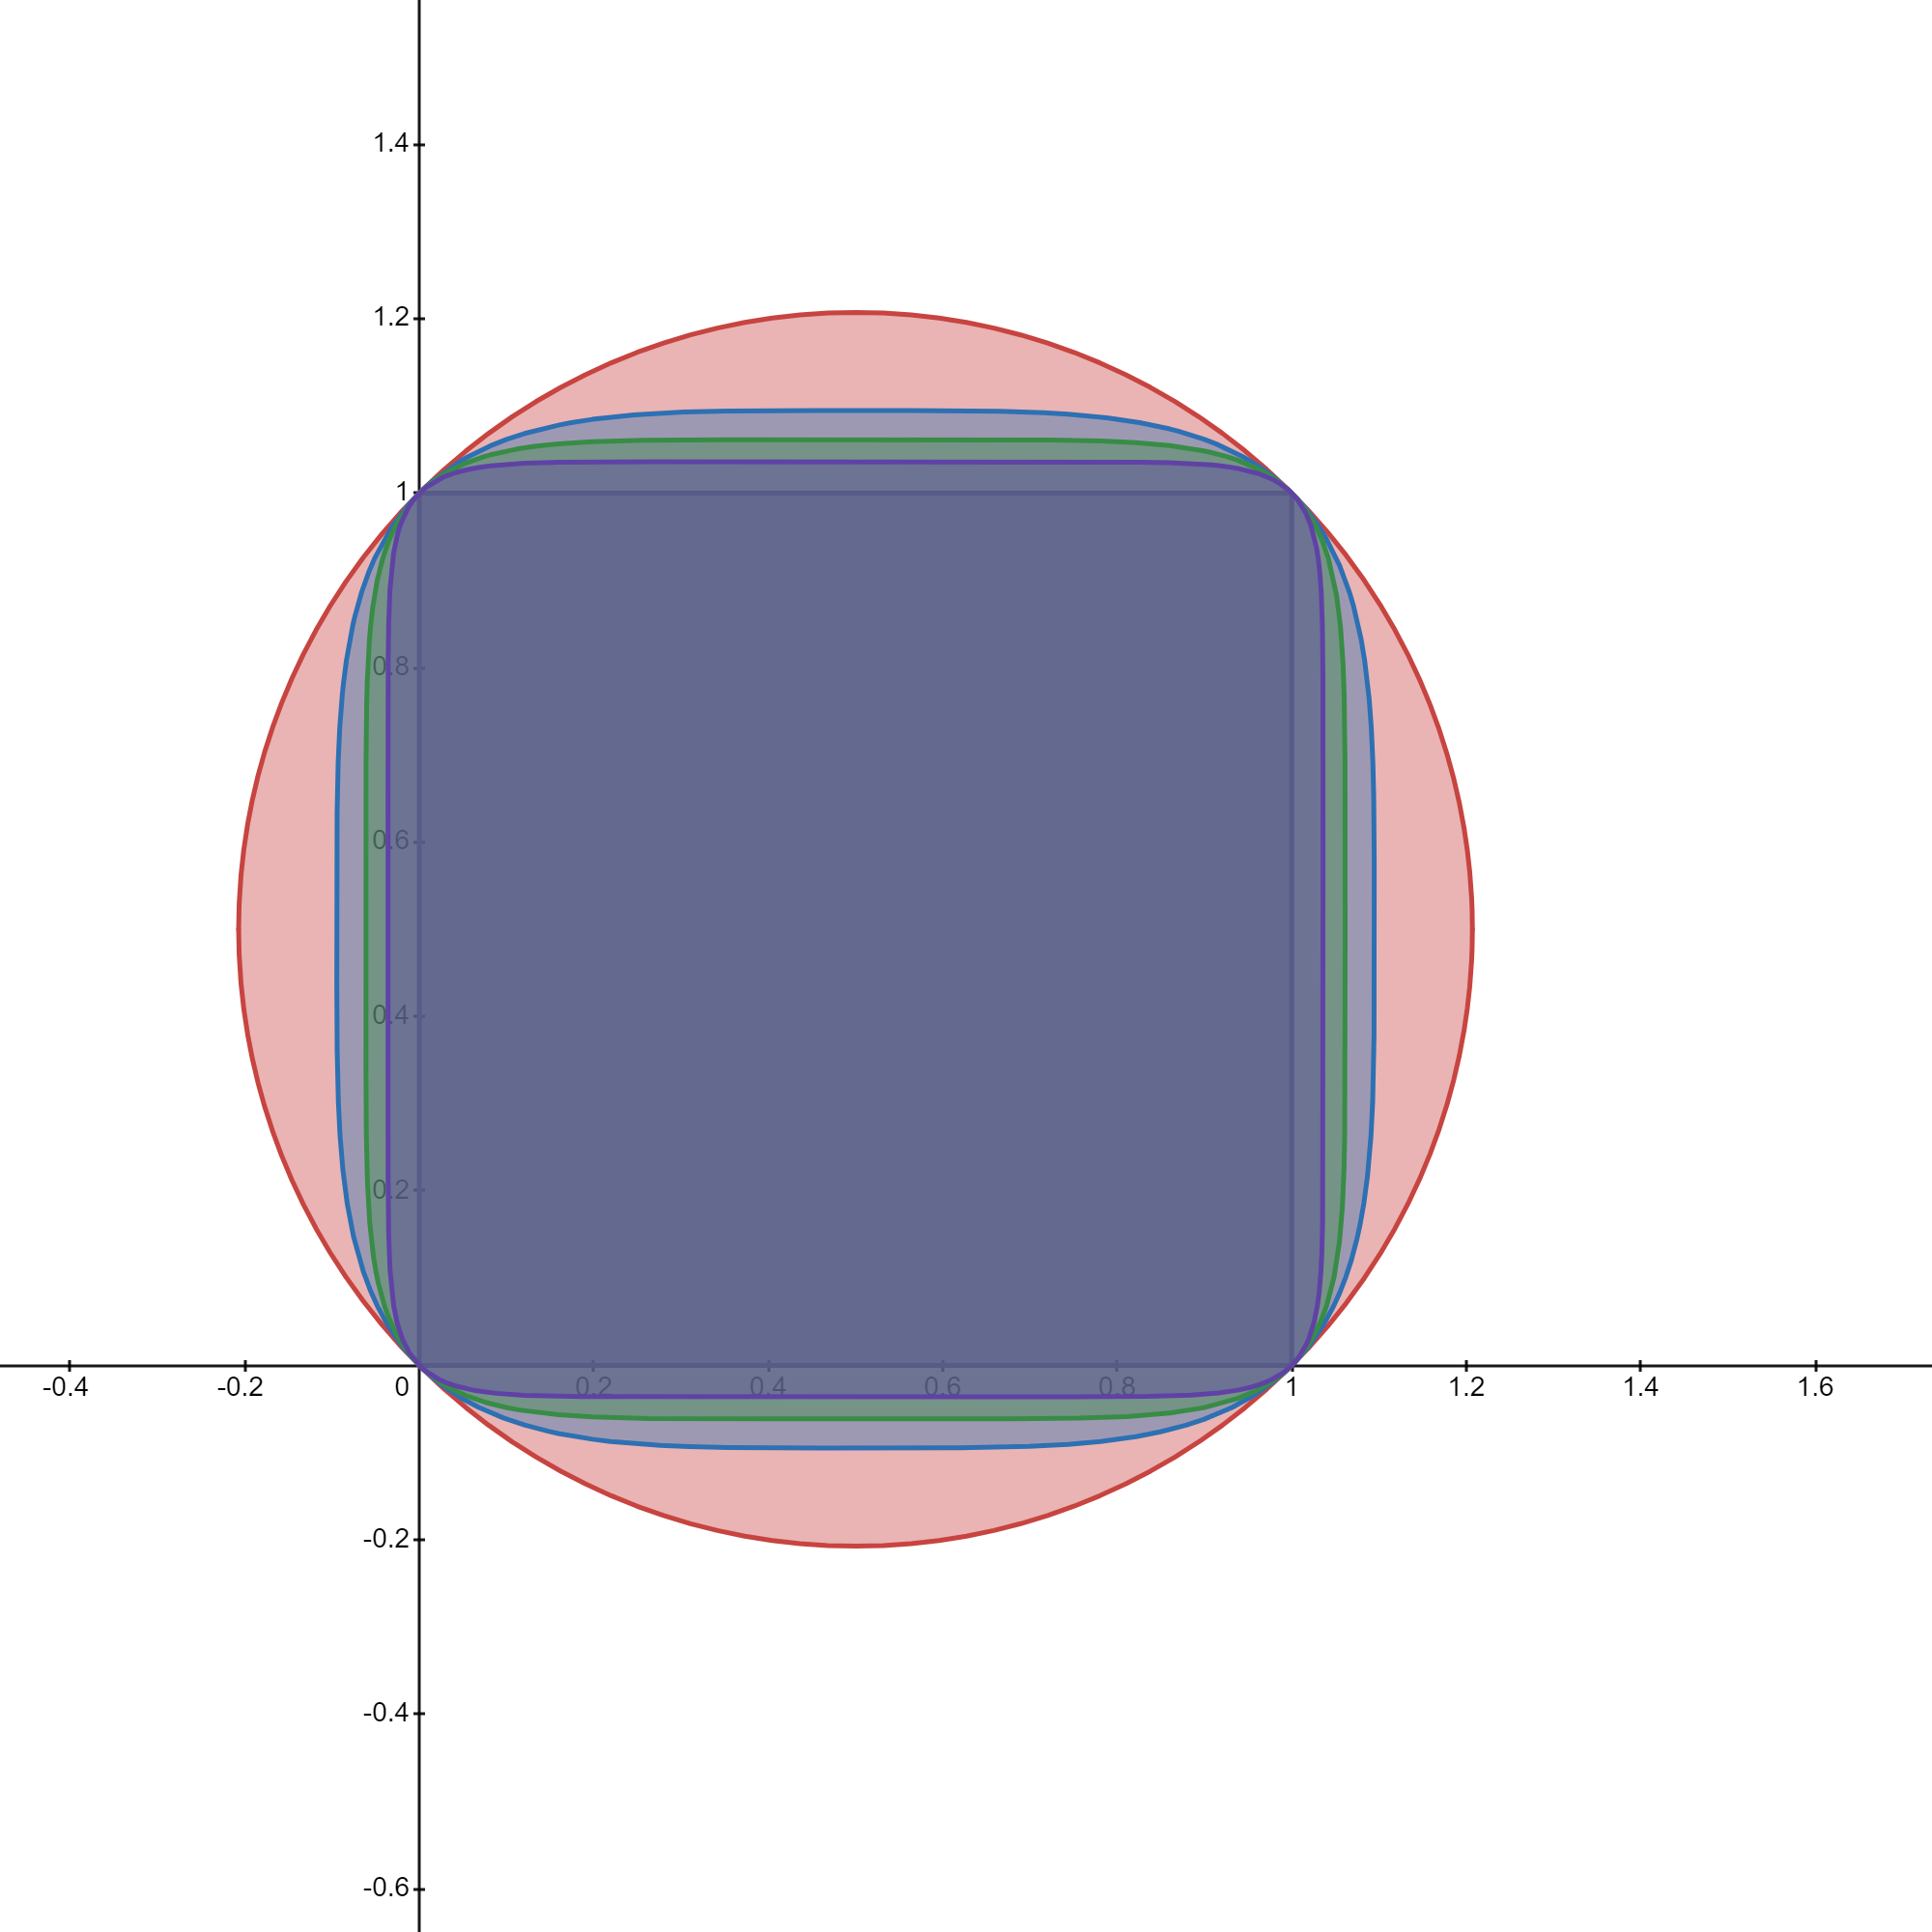
\includegraphics[width=\textwidth]{../figures/desmos_dim_2_v2.png}
		\caption{Feasible Regions $\mathbb{R}^2$}
	\end{subfigure}

	\begin{subfigure}{0.9\textwidth}
		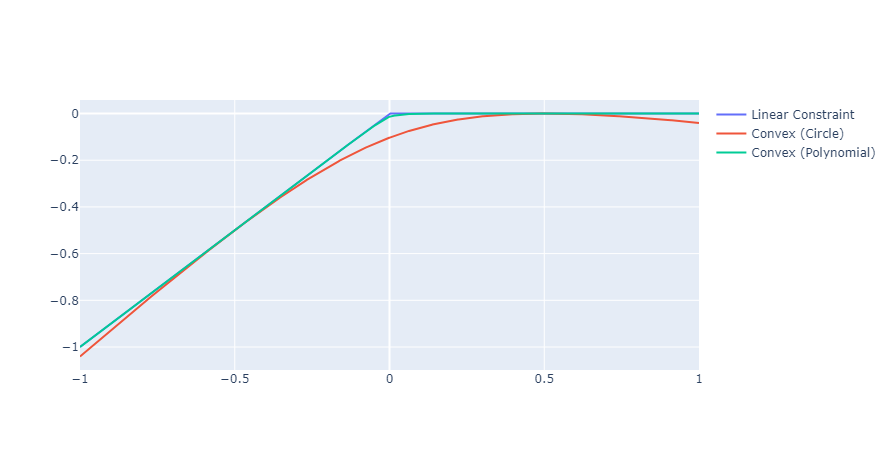
\includegraphics[width=\textwidth]{../figures/value_function_dim_2.png}
		\caption{Value Functions $\mathbb{R}^2$}
	\end{subfigure}
\end{figure}

\begin{figure}
	\centering
	\caption{Feasible Regions and Value Functions in $\mathbb{R}^3$.}\label{fig:feasible_dim_3}

	\begin{subfigure}{0.5\textwidth}
		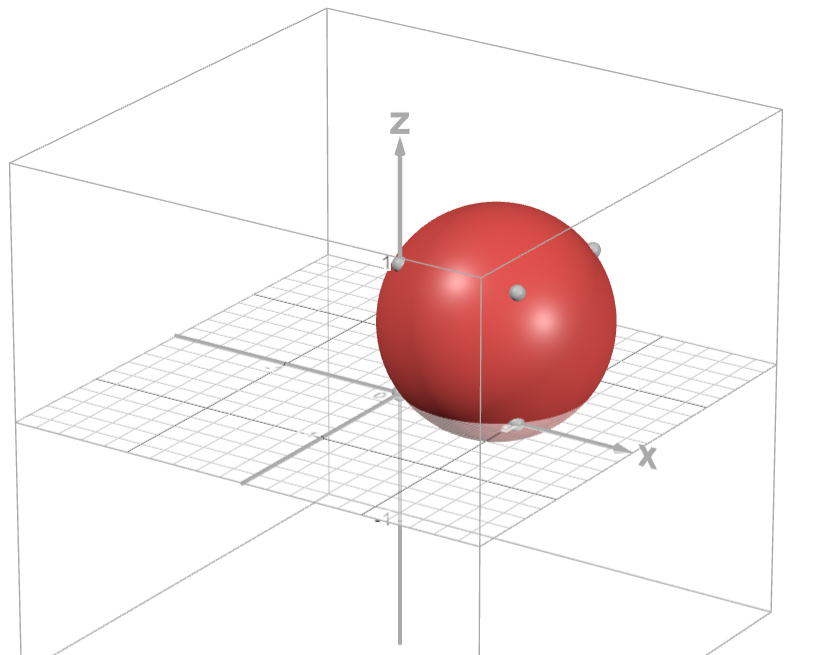
\includegraphics[width=\textwidth]{../figures/desmos_dim_3_unit_ball.png}
		\caption{Unit Cube in $\mathbb{R}^3$}
	\end{subfigure}

	\begin{subfigure}{0.5\textwidth}
		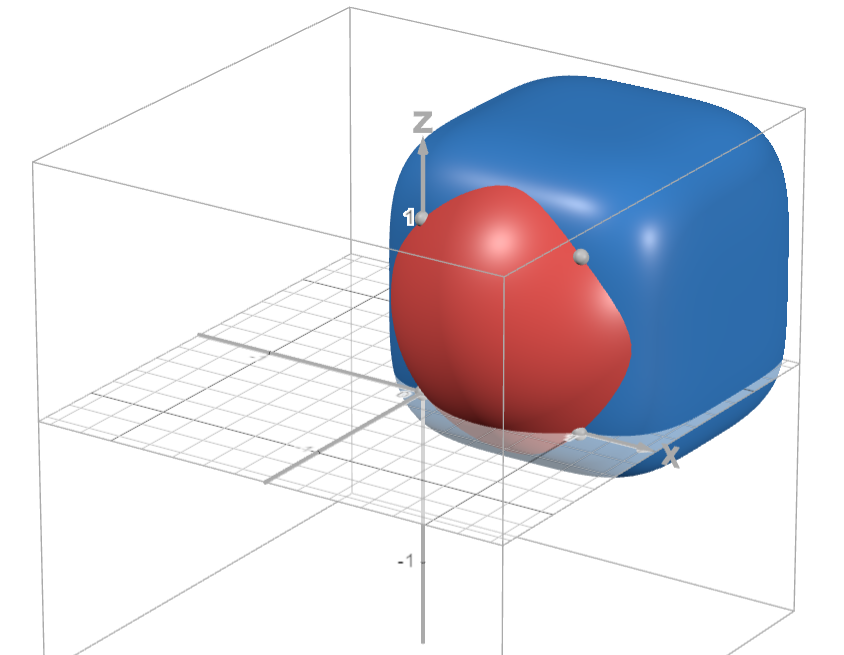
\includegraphics[width=\textwidth]{../figures/desmos_dim_3_unit_ball_and_single_approx.png}
		\caption{(Scaled) Unit Ball and Single Convex Relaxation}
	\end{subfigure}

	\begin{subfigure}{0.5\textwidth}
		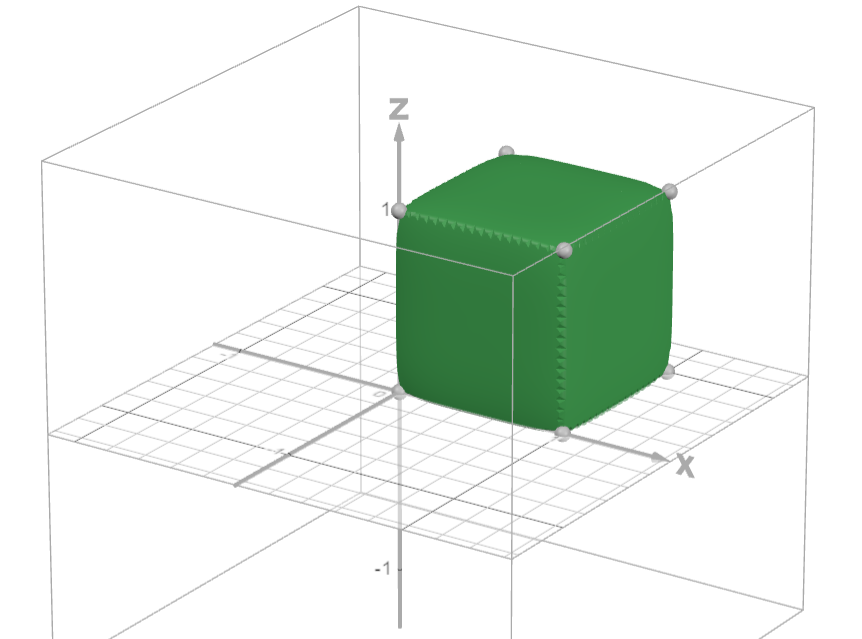
\includegraphics[width=\textwidth]{../figures/desmos_dim_3_poly_shape.png}
		\caption{Full Convex Relaxation}
	\end{subfigure}
\end{figure}



\section{Questions}

\begin{itemize}
	\item Can we get something that is aymptotically exact by letting the approximating feasible region converge? What would the rate requirements be?
	\item Under what conditions is the value function guaranteed to be smooth? For example, $c_2 = 0$ above would not result in a smooth value function.
\end{itemize}

% \bibliographystyle{plain}
% \bibliography{refs.bib}

\end{document}
